\documentclass[12pt]{article}
\usepackage{natbib,amsmath,amsfonts,fullpage,hyphenat,booktabs,graphicx,setspace}
\usepackage[colorlinks,linkcolor=blue,citecolor=blue,urlcolor=blue]{hyperref}
\setcitestyle{square,super,comma}
\onehalfspacing{}

\title{Updated Architecture and agent definition of Baking and Packaging stage\\Multiagent and Agent System}
\author{Arun Prabhu\\Md Zahiduzzaman\\Dharmin Bakaraniya}
\begin{document}
\maketitle{}
\pagebreak
\section{Updated Architecture}%
\label{sec:architecture}

\begin{figure}[htpb]
    \centering
    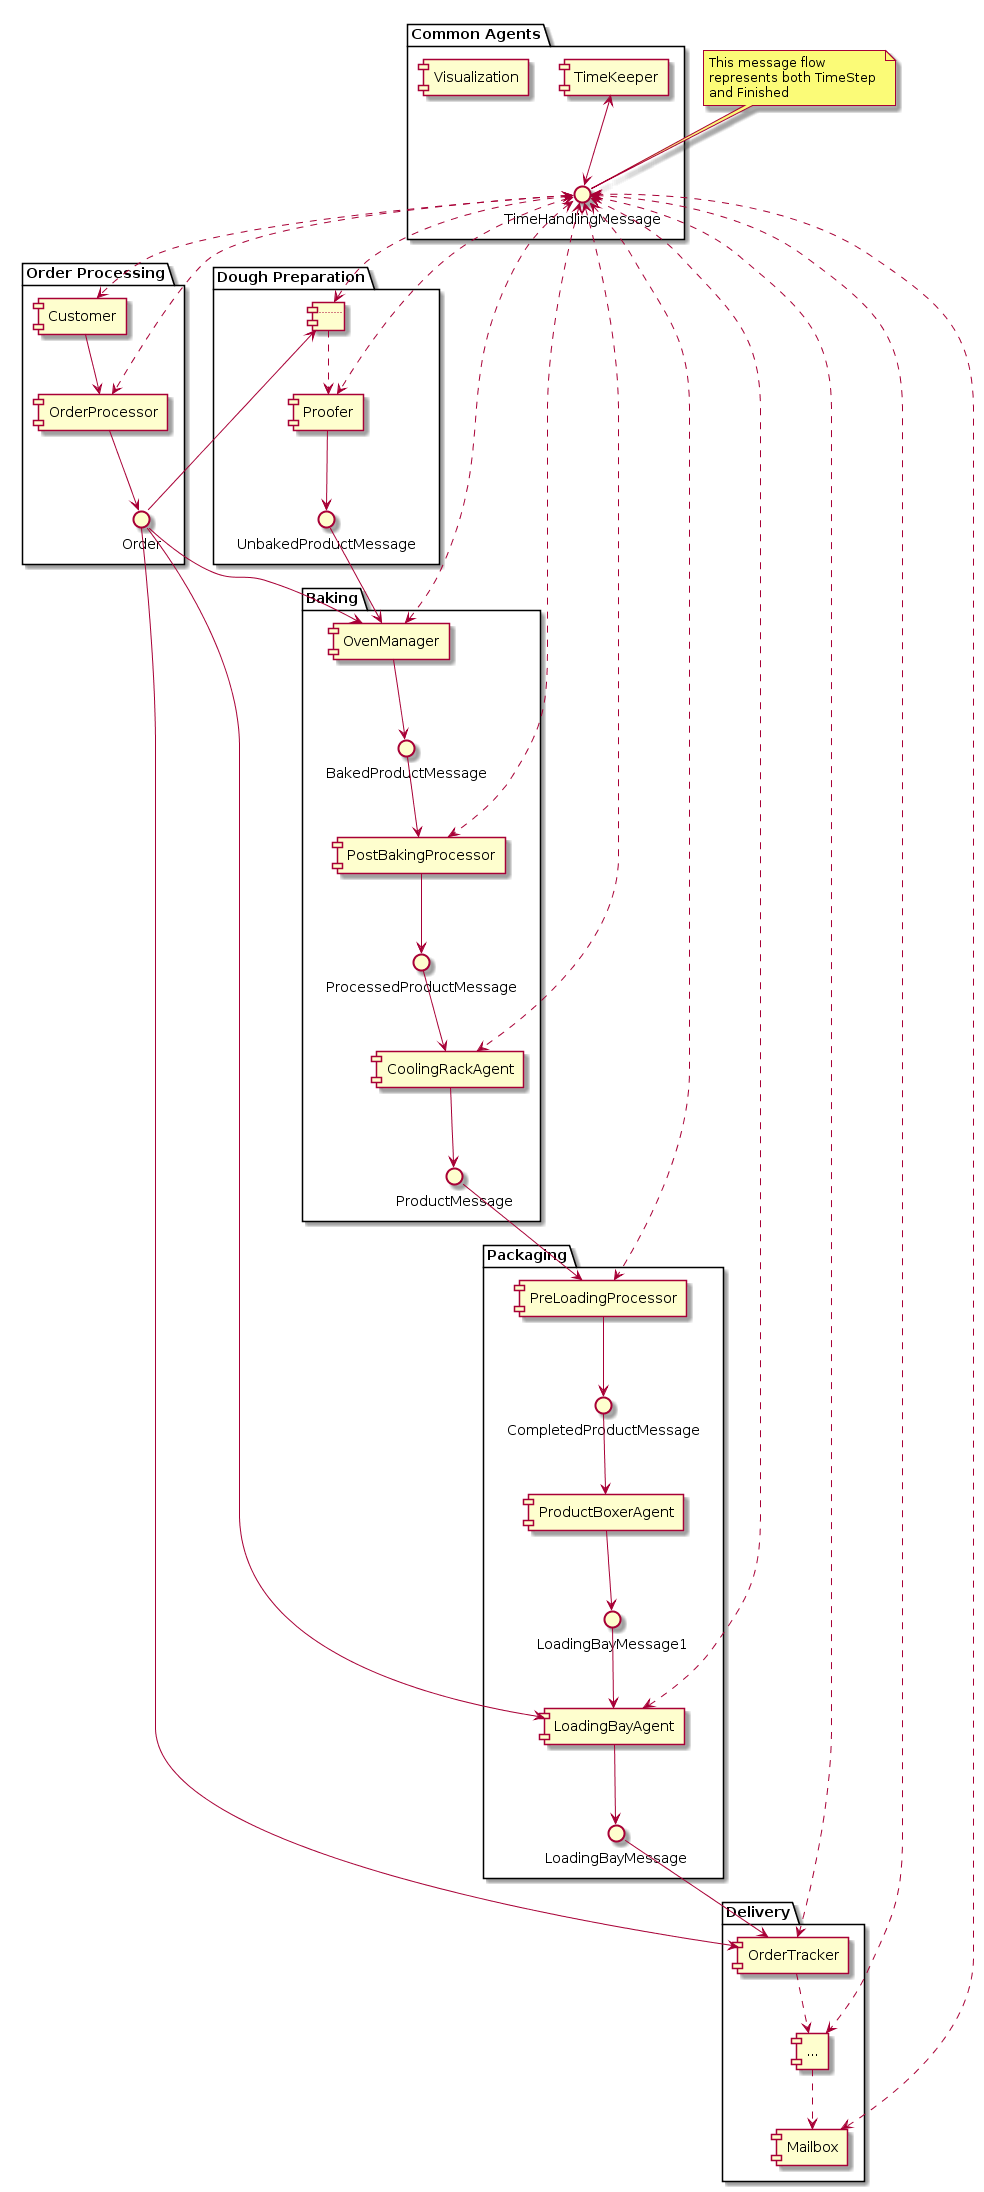
\includegraphics[width=0.46\linewidth]{component_diagram.png}
    \caption{Architecture diagram explaining the interaction between customer and bakery agents}\label{fig:somename}
\end{figure}

\pagebreak

\section{Architectural Description}%
\label{sec:description}
We (right-brothers) are responsible for the Baking and Packaging stages, common agents like BaseAgent and TimeKeeper agent and Order board by stage visualization agent.
\begin{itemize}
\item \textbf{Common Agents}
\begin{itemize}
    \item \textbf{TimeKeeper}: 
 It is responsible for the movement of time in the entire bakery eco-system.
 This is responsible for providing all the other agents with a common time reference so that everyone are in sync except the visualization agents.
 This also gets feedback from all the agents about the status of their tasks.
 If all the agents are done with whatever task they were supposed to finish in the time step, the TimeKeeper increments the time step. 
 It is also responsible for shutting down the platform when the simulation time ends.
\item \textbf{BaseAgent}:
BaseAgent is a parent to all agents in bakery simulation.
It is mainly responsible for registering the agent to yellow pages and talking to TimeKeeper.
It is also responsible for sending the message to visualization agents.
Every agent that inherits BaseAgent only have to call \texttt{finished} when their task is finished for that time step.
\item \textbf{Visualization}:
Visualization agent receives messages from baseAgent of all agents and parses this message to extract whetever information it needs.
It then uses this information to create graphical representation using \texttt{JavaFX}.
\end{itemize}
\item \textbf{Baking Stage Agents}
\begin{itemize}
    \item \textbf{OvenManager}: 
 We assign a single Agent to manage all the ovens in the bakery.
 It receives the Order from OrderProcessor agent. 
 It receives \texttt{UnbakedProductMessage} from \texttt{Proofer}.
 It bakes the products it received from \texttt{Proofer} and sends \texttt{BakedProductMessage} to \texttt{PostBakingProcessor}.
 It agregates products of same type if the product is not being baked. 
    \item \textbf{PostBakingProcessor}:
 It receives \texttt{BakedProductMessage} from \texttt{OvenManager}.
 It processes all the steps in the recipe of that product which occur between \texttt{Baking} and \texttt{Cooling} steps. 
 It sends the \texttt{ProcessedProductMessage} to \texttt{CoolingRackAgent}.
    \item \textbf{CoolingRackAgent}:
 It receives \texttt{ProcessedProductMessage} from \texttt{PostBakingProcessor}.
 It performs cooling step of the recipe corresponding to that product.
 It sends \texttt{ProductMessage} to \texttt{PreLoadingProcessor} in the packaging stage.
\end{itemize}
\item \textbf{Packaging Stage Agents}
\begin{itemize}
    \item \textbf{PreLoadingProcessor}:
 It recieves \texttt{ProductMessage} from \texttt{CoolingRackAgent} from Baking stage.
 It performs all steps in recipe of that product which lie between \texttt{Cooling} and \texttt{Packaging}.
 It sends \texttt{CompletedProductMessage} to \texttt{LoadingBayAgent}.
    \item \textbf{LoadingBayAgent}:
 It recieves \texttt{CompletedProductMessage} from \texttt{PreLoadingProcessor}.
 It prioritizes the pending orders in the todo list according to the earliest order delivery dates. 
 Whenever any product requirement of any order in the todo list becomes available, a \texttt{LoadingBayMessage} is created with that particular product, and is sent to the \texttt{OrderTracking} agent of the \texttt{Delivery Stage}.   
\end{itemize}
\end{itemize}


\newpage{}
\section{Class descriptions}%
\label{sec:agent_descriptions}

\subsection{TimeKeeper}
\begin{itemize}
    \item \textbf{Stage}: Common Agent
    \item \textbf{Agent/Object}: Agent
    \item \textbf{Static/Dynamic}: Static
    \item \textbf{Behaviour}: SendTimeStep (OneShot), TimeStepConfirmationBehaviour (Cyclic)
    \item \textbf{Messages in}: 
        \begin{itemize}
            \item  finished (Sender: all agents)
        \end{itemize}
    \item \textbf{Messages out}:
        \begin{itemize}
            \item  TimeStep (Receiver: all agents)
        \end{itemize}
\end{itemize}
\newpage{}

\subsection{BaseAgent}
\begin{itemize}
    \item \textbf{Stage}: NA
    \item \textbf{Agent/Object}: Agent
    \item \textbf{Static/Dynamic}: Static  
    \item \textbf{Behaviour}: PermitAction (Cyclic)
    \item \textbf{Messages in}:
        \begin{itemize}
            \item  TimeStep (Sender: TimeKeeper)
        \end{itemize}
    \item \textbf{Messages out}:
        \begin{itemize}
            \item  finished (Receiver: TimeKeeper)
            \item  all messages(Receiver: Visualization Agents)
        \end{itemize}
\end{itemize}
\newpage{}

\subsection{Visualization agent}
\begin{itemize}
    \item \textbf{Stage}: Common Agents 
    \item \textbf{Agent/Object}: Agent
    \item \textbf{Static/Dynamic}: Static
    \item \textbf{Behaviour}: MessageServer (Cyclic)
    \item \textbf{Messages in}:
        \begin{itemize}
            \item  all messages (Sender: all agents)
        \end{itemize}
\end{itemize}
\newpage{}

\subsection{OvenManager}
\begin{itemize}
    \item \textbf{Stage}: Baking 
    \item \textbf{Agent/Object}: Agent 
    \item \textbf{Static/Dynamic}: Static
    \item \textbf{Behaviour}: Bake (Cyclic), OrderServer (Cyclic), UnbakedProductsServer (Cyclic) 
    \item \textbf{Messages in}:
        \begin{itemize}
            \item  Order (Sender: OrderProcessor)
            \item  UnbakedProductMessage (Sender: Proofer)
        \end{itemize}
    \item \textbf{Messages out}:
        \begin{itemize}
            \item  BakedProductMessage (Receiver: PostBakingProcessor)
        \end{itemize}
\end{itemize}
\newpage{}

\subsection{PostBakingProcessor}
\begin{itemize}
    \item \textbf{Stage}: Baking
    \item \textbf{Agent/Object}: Agent 
    \item \textbf{Static/Dynamic}: Static
    \item \textbf{Behaviour}: BakedProductsServer (Cyclic), Process (Cyclic)
    \item \textbf{Messages in}:
        \begin{itemize}
            \item  BakedProductMessage (Sender: OvenManager)
        \end{itemize}
    \item \textbf{Messages out}:
        \begin{itemize}
            \item  ProcessedProductMessage (Receiver: CoolingRackAgent)
        \end{itemize}
\end{itemize}
\newpage{}

\subsection{CoolingRackAgent}
\begin{itemize}
    \item \textbf{Stage}: Baking
    \item \textbf{Agent/Object}: Agent
    \item \textbf{Static/Dynamic}: Static
    \item \textbf{Behaviour}: ProcessedProductServer (Cyclic), CoolProducts (Cyclic)
    \item \textbf{Messages in}:
        \begin{itemize}
            \item ProcessedProductMessage (Sender: PostBakingProcessor)
        \end{itemize}
    \item \textbf{Messages out}:
        \begin{itemize}
            \item ProductMessage (Receiver: PreLoadingProcessor)
        \end{itemize}
\end{itemize}
\newpage{}

\subsection{PreLoadingProcessor}
\begin{itemize}
    \item \textbf{Stage}: Packaging
    \item \textbf{Agent/Object}: Agent
    \item \textbf{Static/Dynamic}: Static
    \item \textbf{Behaviour}: Process (Cyclic), CooledProductServer (Cyclic), OrderServer (Cyclic)
    \item \textbf{Messages in}:
        \begin{itemize}
            \item ProductMessage (Sender: CoolingRackAgent)
            \item Order (Sender: OrderProcessor)
        \end{itemize}
    \item \textbf{Messages out}:
        \begin{itemize}
            \item CompletedProductMessage (Receiver: LoadingBayAgent)
        \end{itemize}
\end{itemize}
\newpage{}

\subsection{LoadingBayAgent}
\begin{itemize}
    \item \textbf{Stage}: Packaging
    \item \textbf{Agent/Object}: Agent
    \item \textbf{Static/Dynamic}: Static
    \item \textbf{Behaviour}: OrderReceiver (Cyclic), CompletedProductReceiver (Cyclic)
    \item \textbf{Messages in}:
        \begin{itemize}
            \item CompletedProductMessage (Sender: PreLoadingProcessor)
        \end{itemize}
    \item \textbf{Messages out}:
        \begin{itemize}
            \item LoadingBayMessage (Receiver: OrderTracker)
        \end{itemize}
\end{itemize}

\end{document}

